% defer/hazptr.tex
% mainfile: ../perfbook.tex
% From an C++ Standards Committee meeting:  "Can I hazptr cheezeberger?"

\section{Hazard Pointers}
\label{sec:defer:Hazard Pointers}
%
\epigraph{If in doubt, turn it inside out.}{\emph{Zara Carpenter}}

동시적 레퍼런스 카운팅의 문제를 막는 한가지 방법은 레퍼런스 카운터를 뒤집어
구현하는 것으로, 즉, 데이터 원소에 저장된 정수의 값을 증가시키는 대신 CPU별
(또는 쓰레드별) 리스트에 데이터 원소로의 포인터를 저장하는 것입니다.
이 리스트의 각 원소는 \emph{해저드 포인터}~\cite{MagedMichael04a} 라고
불립니다.\footnote{
	독립적으로 다른 사람들에 의해서도 발명되었습니다~\cite{HerlihyLM02}.}
그러면 주어진 데이터 원소의 ``가상 레퍼런스 카운터'' 의 값은 이 원소를 참조하는
해저드 포인터의 갯수를 세는 것으로 구해질 수 있습니다.
따라서, 이 원소가 읽기 쓰레드에 의해 액세스 될 수 없게 되다면, 해당 원소를
참조하는 해저드 포인터가 더이상 존재하지 않게 되어서, 이 원소는 안전히 메모리
해제될 수 있습니다.

\iffalse

One way of avoiding problems with concurrent reference counting
is to implement the reference counters
inside out, that is, rather than incrementing an integer stored in the
data element, instead store a pointer to that data element in
per-CPU (or per-thread) lists.
Each element of these lists is called a
\emph{hazard pointer}~\cite{MagedMichael04a}.\footnote{
	Also independently invented by others~\cite{HerlihyLM02}.}
The value of a given data element's ``virtual reference counter'' can
then be obtained by counting the number of hazard pointers referencing
that element.
Therefore, if that element has been rendered inaccessible to readers,
and there are no longer any hazard pointers referencing it, that element
may safely be freed.

\fi

\begin{listing}[tbp]
\input{CodeSamples/defer/hazptr@record_clear.fcv}
\caption{Hazard-Pointer Recording and Clearing}
\label{lst:defer:Hazard-Pointer Recording and Clearing}
\end{listing}

물론, 이는 해저드 포인터 획득이 동시의 삭제와의 위험한 레이스를 막기 위해 아주
조심스럽게 다뤄져야 함을 의미합니다.
\begin{fcvref}[ln:defer:hazptr:record_clear]
Listing~\ref{lst:defer:Hazard-Pointer Recording and Clearing}
에 하나의 구현이 보여져 있는데, \clnrefrange{htr:b}{htr:e} 에
\co{hp_try_record()} 가, \clnrefrange{hr:b}{hr:e} 에 \co{hp_record()} 가,
그리고 \clnrefrange{hc:b}{hc:e} 에 \co{hp_clear()} 가 있습니다
(\path{hazptr.h}).

라인~\lnref{htr:e} 의 \co{hp_try_record()} 매크로는 \co{_h_t_r_impl()} 함수를
위한 캐스팅 래퍼로, \co{p} 에 의해 참조되는 포인터를 \co{hp} 에 의해 참조되는
해저드 포인터에 저장합니다.
이게 성공하면, 저장된 포인터의 값을 리턴합니다.
해당 포인터가 \co{NULL} 이 되는 관계로 여기 실패하면, \co{NULL} 을 리턴합니다.
마지막으로, 업데이트와의 레이스 때문에 실패하면 특수한 \co{HAZPTR_POISON}
토큰을 리턴합니다.

\iffalse

Of course, this means that hazard-pointer acquisition must be carried
out quite carefully in order to avoid destructive races with concurrent
deletion.
\begin{fcvref}[ln:defer:hazptr:record_clear]
One implementation is shown in
Listing~\ref{lst:defer:Hazard-Pointer Recording and Clearing},
which shows \co{hp_try_record()} on \clnrefrange{htr:b}{htr:e},
\co{hp_record()} on \clnrefrange{hr:b}{hr:e}, and
\co{hp_clear()} on
\clnrefrange{hc:b}{hc:e} (\path{hazptr.h}).

The \co{hp_try_record()} macro on line~\lnref{htr:e} is simply a casting
wrapper for the \co{_h_t_r_impl()} function, which attempts to store
the pointer referenced by \co{p} into the hazard pointer referenced
by \co{hp}.
If successful, it returns the value of the stored pointer.
If it fails due to that pointer being \co{NULL}, it returns \co{NULL}.
Finally, if it fails due to racing with an update, it returns a special
\co{HAZPTR_POISON} token.

\fi

\QuickQuiz{
	해저드 포인터 논문들은 삭제된 원소들을 표시하기 위해 각 포인터의 바닥
	비트들을 사용하는데 \co{HAZPTR_POISON} 은 왜 사용되나요?

	\iffalse

	Given that papers on hazard pointers use the bottom bits
	of each pointer to mark deleted elements, what is up with
	\co{HAZPTR_POISON}?

	\fi

}\QuickQuizAnswer{
	해저드 포인트의 해당 공개된 구현은 삽입과 삭제에 non-blocking 동기화
	기법을 사용했습니다.
	이 기법들은 이 데이터 구조를 횡단하는 읽기 쓰레드가 업데이트 쓰레드가
	업데이트를 완료하는 것을 ``도와줄'' 것을 필요로 하는데 이는 읽기
	쓰레드들이 삭제된 원소의 다음 원소를 봐야 함을 의미합니다.

	대조적으로, 우린 업데이트들을 동기화 하기 위해 락킹을 사용할텐데, 이는
	읽기 쓰레드들이 업데이트 쓰레드들의 업데이트 완료를 도울 필요를
	없애버려서 결국 우리가 포인터의 바닥 비트를 그대로 둘 수 있게 해줍니다.
	이 방법은 읽기 쪽 코드를 더 간단하고 빠르게 해줍니다.

	\iffalse

	The published implementations of hazard pointers used
	non-blocking synchronization techniques for insertion
	and deletion.
	These techniques require that readers traversing the
	data structure ``help'' updaters complete their updates,
	which in turn means that readers need to look at the successor
	of a deleted element.

	In contrast, we will be using locking to synchronize updates,
	which does away with the need for readers to help updaters
	complete their updates, which in turn allows us to leave
	pointers' bottom bits alone.
	This approach allows read-side code to be simpler and faster.

	\fi

}\QuickQuizEnd

라인~\lnref{htr:ro1} 은 보호되어야 할 객체로의 포인터를 읽습니다.
라인~\lnref{htr:race1} 이 이 포인터가 \co{NULL} 이거나 특수한 삭제된 객체
토큰인 \co{HAZPTR_POISON} 이었음을 발견하게 되면, 호출자에게 실패를 알리기 위해
이 포인터의 값을 리턴합니다.
그렇지 않다면, 라인~\lnref{htr:store} 는 명시된 해저드 포인터에 이 포인터를
저장하고, 라인~\lnref{htr:mb} 는 라인~\lnref{htr:ro2} 에서의 원래 포인터의 다시
읽기와 이 저장 사이의 순서를 완전히 강제합니다.
(메모리 순서 규칙에 대한 더 많은 내용을 위해선
Chapter~\ref{chp:Advanced Synchronization: Memory Ordering} 를 참고하시기
바랍니다.)
원래 포인터의 값이 변경되지 않았다면, 이 해저드 포인터는 가리켜진 객체를
보호하고, 이 경우 라인~\lnref{htr:success} 는 이 객체로의 포인터를 리턴하는데,
이는 또한 호출자에게 성공을 알립니다.
그렇지 않고, 이 포인터가 두개의 \co{READ_ONCE()} 사이에서 변경되었다면,
라인~\lnref{htr:race2} 는 실패를 알립니다.

\iffalse

Line~\lnref{htr:ro1} reads the pointer to the object to be protected.
If line~\lnref{htr:race1} finds that this pointer was either \co{NULL} or
the special \co{HAZPTR_POISON} deleted-object token, it returns
the pointer's value to inform the caller of the failure.
Otherwise, line~\lnref{htr:store} stores the pointer into the specified
hazard pointer, and line~\lnref{htr:mb} forces full ordering of that
store with the reload of the original pointer on line~\lnref{htr:ro2}.
(See Chapter~\ref{chp:Advanced Synchronization: Memory Ordering}
for more information on memory ordering.)
If the value of the original pointer has not changed, then the hazard
pointer protects the pointed-to object, and in that case,
line~\lnref{htr:success} returns a pointer to that object, which also
indicates success to the caller.
Otherwise, if the pointer changed between the two \co{READ_ONCE()}
invocations, line~\lnref{htr:race2} indicates failure.

\fi

\QuickQuiz{
	Listing~\ref{lst:defer:Hazard-Pointer Recording and Clearing}
	의 \co{hp_try_record()} 는 왜 데이터 원소로의 이중 간접 경로를 갖나요?
	\co{void **} 대신 \co{void *} 를 쓰는게 어떻습니까?

	\iffalse

	Why does \co{hp_try_record()} in
	Listing~\ref{lst:defer:Hazard-Pointer Recording and Clearing}
	take a double indirection to the data element?
	Why not \co{void *} instead of \co{void **}?

	\fi

}\QuickQuizAnswer{
	\co{hp_try_record()} 는 동시의 수정을 검사해야만 하기 때문입니다.
	이 일을 하기 위해선 이 원소로의 포인터로의 변경을 검사하기 위해 이
	원소로의 포인터로의 포인터를 필요로 합니다.

	\iffalse

	Because \co{hp_try_record()} must check for concurrent modifications.
	To do that job, it needs a pointer to a pointer to the element,
	so that it can check for a modification to the pointer to the
	element.

	\fi

}\QuickQuizEnd

\co{hp_record()} 함수는 상당히 단순합니다: 리턴 값이 \co{HAZPTR_POISON} 이 아닌
무엇인가일 때까지 반복적으로 \co{hp_try_record()} 를 호출합니다.

\iffalse

The \co{hp_record()} function is quite straightforward: It repeatedly
invokes \co{hp_try_record()} until the return value is something other
than \co{HAZPTR_POISON}.

\fi

\QuickQuiz{
	왜 \co{hp_try_record()} 를 신경쓰죠?
	그냥 실패에 내성 있는 \co{hp_record()} 함수를 그냥 사용하는게 더 쉽지
	않나요?

	\iffalse

	Why bother with \co{hp_try_record()}?
	Wouldn't it be easier to just use the failure-immune
	\co{hp_record()} function?

	\fi

}\QuickQuizAnswer{
	어떤 측면에선 그게 더 쉬울 수도 있습니다만, Pre-BSD 라우팅 예에서 곧
	보겠지만, \co{hp_record()} 는 단순하게 동작하지 않는 상황이 있습니다.

	\iffalse

	It might be easier in some sense, but as will be seen in the
	Pre-BSD routing example, there are situations for which
	\co{hp_record()} simply does not work.

	\fi

}\QuickQuizEnd

\co{hp_clear()} 함수는 심지어 더 간단한데, 이 해저드 포인터에 의해 보호되는
객체의 호출자의 사용과 이 해저드 포인터를 \co{NULL} 로 만드는 것 사이의 완전한
순서를 강제하기 위해 \co{smp_mb()} 가 사용됩니다.
\end{fcvref}

\iffalse

The \co{hp_clear()} function is even more straightforward, with
an \co{smp_mb()} to force full ordering between the caller's uses
of the object protected by the hazard pointer and the setting of
the hazard pointer to \co{NULL}.
\end{fcvref}

\fi

\begin{listing}[tbp]
\input{CodeSamples/defer/hazptr@scan_free.fcv}
\caption{Hazard-Pointer Scanning and Freeing}
\label{lst:defer:Hazard-Pointer Scanning and Freeing}
\end{listing}

\begin{fcvref}[ln:defer:hazptr:scan_free:free]
해저드 포인터로 보호되는 객체가 연결된 데이터 구조에서 일단 제거되어서 미래의
해저드 포인터 사용 읽기 쓰레드들에게 접근될 수 없게 되면, 그 객체는
Listing~\ref{lst:defer:Hazard-Pointer Scanning and Freeing}
(\path{hazptr.c}) 의 \clnrefrange{b}{e} 에 보인 \co{hazptr_free_later()} 로
넘겨집니다.
라인~\lnref{enq:b} 와~\lnref{enq:e} 는 이 객체를 쓰레드별 리스트 \co{rlist} 에
넣고 라인~\lnref{count} 에서 \co{rcount} 에 이 객체의 수를 셉니다.
라인~\lnref{check} 가 충분히 많은 수의 객체들이 이제 들어와 있다는 것을 보게
되면, 라인~\lnref{scan} 은 그 중 일부를 메모리 해제하기 위해 \co{hazptr_scan()}
을 호출합니다.
\end{fcvref}

\iffalse

\begin{fcvref}[ln:defer:hazptr:scan_free:free]
Once a hazard-pointer-protected object has been removed from its
linked data structure, so that it is now inaccessible to future
hazard-pointer readers, it is passed to \co{hazptr_free_later()},
which is shown on \clnrefrange{b}{e} of
Listing~\ref{lst:defer:Hazard-Pointer Scanning and Freeing}
(\path{hazptr.c}).
Lines~\lnref{enq:b} and~\lnref{enq:e}
enqueue the object on a per-thread list \co{rlist}
and line~\lnref{count} counts the object in \co{rcount}.
If line~\lnref{check} sees that a sufficiently large number of objects are now
queued, line~\lnref{scan} invokes \co{hazptr_scan()} to attempt to
free some of them.
\end{fcvref}

\fi

\begin{fcvref}[ln:defer:hazptr:scan_free:scan]
이 리스팅의 \clnrefrange{b}{e} 에 \co{hazptr_scan()} 함수가 보여져 있습니다.
이 함수는 고정된 쓰레드의 최대 갯수 (\co{NR_THREADS}) 와 고정된 크기의 해저드
포인터 배열이 사용될 수 있게끔 하는 쓰레드당 해저드 포인터의 고정된 최대 갯수
(\co{K}) 에 의존하고 있습니다.
어떤 쓰레드든 이 해저드 포인터들을 스캔해야 할 수 있으므로,  각 쓰레드는 각자의
배열을 가지고 있는데, 이는 쓰레드별 변수 \co{gplist} 를 통해 참조됩니다.
라인~\lnref{check} 가 이 쓰레드는 아직 자신의 \co{gplist} 를 할당받지 않았음을
알게 되면, \clnrefrange{alloc:b}{alloc:e} 가 이 할당을 진행합니다.
라인~\lnref{mb1} 에서의 메모리 배리어는 이 쓰레드에 의한 모든 객체의 제거가
\clnrefrange{loop:b}{loop:e} 가 모든 해저드 포인터를 스캔하고 NULL 이 아닌
포인터들을 \co{plist} 배열에 넣고 \co{psize} 에 그 수를 세기 전에 볼 수 있음을
보장하게 합니다.
라인~\lnref{mb2} 에서의 메모리 배리어는 이 해저드 포인터들의 읽기가 어떤 객체의
메모리 해제보다도 먼저 일어날 것을 보장되게 합니다.
라인~\lnref{sort} 는 이어서 이 배열을 정렬해서 아래의 바이너리 탐색이 가능하게
합니다.

\iffalse

\begin{fcvref}[ln:defer:hazptr:scan_free:scan]
The \co{hazptr_scan()} function is shown on \clnrefrange{b}{e}
of the listing.
This function relies on a fixed maximum number of threads (\co{NR_THREADS})
and a fixed maximum number of hazard pointers per thread (\co{K}),
which allows a fixed-size array of hazard pointers to be used.
Because any thread might need to scan the hazard pointers, each thread
maintains its own array, which is referenced by the per-thread variable
\co{gplist}.
If line~\lnref{check} determines that this thread has not yet allocated its
\co{gplist}, \clnrefrange{alloc:b}{alloc:e} carry out the allocation.
The memory barrier on line~\lnref{mb1} ensures that all threads see the
removal of all objects by this thread before
\clnrefrange{loop:b}{loop:e} scan
all of the hazard pointers, accumulating non-NULL pointers into
the \co{plist} array and counting them in \co{psize}.
The memory barrier on line~\lnref{mb2} ensures that the reads of
the hazard pointers
happen before any objects are freed.
Line~\lnref{sort} then sorts this array to enable use of binary search below.

\fi

라인~\lnref{rem:b} 와~\lnref{rem:e} 는 이 쓰레드의 곧 메모리 해제할 객체들
리스트의 모든 원소들을 제거하고, 그것들을 지역적인 \co{tmplist} 에 위치시킨 후
라인~\lnref{zero} 에서 그 수를 0으로 만듭니다.
\Clnrefrange{loop2:b}{loop2:e} 에 있는 반복문의 각 수행에서는 곧 메모리 해제될
객체들 각각을 처리합니다.
라인~\lnref{rem1st:b} 와~\lnref{rem1st:e} 는 \co{tmplist} 에서 첫번째 객체를
제거하고, 라인~\lnref{chkhazp:b} 와~\lnref{chkhazp:e} 는 이 객체를 보호하는
해저드 포인터가 있음을 확인하고, \clnrefrange{back:b}{back:e} 는 그것을
\co{rlist} 에 되돌려 놓습니다.
그렇지 않으면, 라인~\lnref{free} 는 이 객체를 메모리 해제합니다.
\end{fcvref}

\iffalse

Lines~\lnref{rem:b} and~\lnref{rem:e}
remove all elements from this thread's list of
to-be-freed objects, placing them on the local \co{tmplist}
and line~\lnref{zero} zeroes the count.
Each pass through the loop spanning
\clnrefrange{loop2:b}{loop2:e} processes each
of the to-be-freed objects.
Lines~\lnref{rem1st:b} and~\lnref{rem1st:e}
remove the first object from \co{tmplist},
and if lines~\lnref{chkhazp:b} and~\lnref{chkhazp:e}
determine that there is a hazard pointer
protecting this object, \clnrefrange{back:b}{back:e}
place it back onto \co{rlist}.
Otherwise, line~\lnref{free} frees the object.
\end{fcvref}

\fi

\begin{listing}[tbp]
\input{CodeSamples/defer/route_hazptr@lookup.fcv}
\caption{Hazard-Pointer Pre-BSD Routing Table Lookup}
\label{lst:defer:Hazard-Pointer Pre-BSD Routing Table Lookup}
\end{listing}

Pre-BSD 라우팅 예제는 데이터 구조와 \co{route_lookup()} 을 위해
Listing~\ref{lst:defer:Hazard-Pointer Pre-BSD Routing Table Lookup}
에 보인 것처럼, \co{route_add()} 와 \co{route_del()} 을 위해선
Listing~\ref{lst:defer:Hazard-Pointer Pre-BSD Routing Table Add/Delete}
에 보인 것처럼 해저드 포인터를 사용할 수 있습니다 (\path{route_hazptr.c}).
레퍼런스 카운팅에서와 같이, 이 해저드 포인터 구현은
page~\pageref{lst:defer:Sequential Pre-BSD Routing Table}
의
Listing~\ref{lst:defer:Sequential Pre-BSD Routing Table}
에 보인 순차적 알고리즘과 상당히 비슷해서 여기선 차이점만 이야기 하겠습니다.

\iffalse

The Pre-BSD routing example can use hazard pointers as shown in
Listing~\ref{lst:defer:Hazard-Pointer Pre-BSD Routing Table Lookup}
for data structures and \co{route_lookup()}, and in
Listing~\ref{lst:defer:Hazard-Pointer Pre-BSD Routing Table Add/Delete}
for \co{route_add()} and \co{route_del()}
(\path{route_hazptr.c}).
As with reference counting, the hazard-pointers implementation
is quite similar to the sequential algorithm shown in
Listing~\ref{lst:defer:Sequential Pre-BSD Routing Table}
on
page~\pageref{lst:defer:Sequential Pre-BSD Routing Table},
so only differences will be discussed.

\fi

\begin{fcvref}[ln:defer:route_hazptr:lookup]
Listing~\ref{lst:defer:Hazard-Pointer Pre-BSD Routing Table Lookup}
부터 시작하면, 라인~\lnref{hh} 는 해저드 포인터 해제를 기다리는 객체들을
리스트에 넣는데 사용되는 \co{->hh} 필드를 보이며, 라인~\lnref{re_freed} 는
미모리 해제 후 사용 버그를 감지하기 위한 \co{->re_freed} 필드를 보이고,
라인~\lnref{tryrecord} 는 해저드 포인터 획득을 시도하기 위해
\co{hp_try_record()} 를 호출합니다.
리턴값이 \co{NULL} 이면, 라인~\lnref{NULL} 은 호출자에게 찾지 못했음을
리턴합니다.
\co{hp_try_record()} 호출이 삭제와 레이스 상태에 빠진다면, 라인~\lnref{deleted}
는 라인~\lnref{retry} 의 \co{retry} 로 돌아와 이 리스트를 시작부터 다시
순회합니다.
\co{do}--\co{while} 루프는 희망한 원소가 찾아질 때까지 돌아가는데, 만약 이
원소가 이미 메모리 해제되어 있다면 라인~\lnref{abort} 가 이 프로그램을
종료시킵니다.
그렇지 않다면, 이 원소의 \co{->iface} 필드가 호출자에게 리턴됩니다.

라인~\lnref{tryrecord} 는 사용하기 더 쉬운 \co{hp_record()} 대신
\co{hp_try_record()} 를 호출해서 \co{hp_try_record()} 의 실패 시에는 전체
탐색을 재시작합니다.
그리고 그런 재시작은 정확성을 위해 분명 필요합니다.
이를 보기 위해, 원소~A, B, 그리고~C 를 담고 있으며 다음 이벤트를 겪는 해저드
포인터로 보호되는 링크드 리스트를 생각해 봅시다:
\end{fcvref}

\iffalse

\begin{fcvref}[ln:defer:route_hazptr:lookup]
Starting with
Listing~\ref{lst:defer:Hazard-Pointer Pre-BSD Routing Table Lookup},
line~\lnref{hh} shows the \co{->hh} field used to queue objects pending
hazard-pointer free,
line~\lnref{re_freed} shows the \co{->re_freed} field used to detect
use-after-free bugs, and line~\lnref{tryrecord} invokes
\co{hp_try_record()} to attempt to acquire a hazard pointer.
If the return value is \co{NULL}, line~\lnref{NULL} returns a not-found
indication to the caller.
If the call to \co{hp_try_record()} raced with deletion, line~\lnref{deleted}
branches back to line~\lnref{retry}'s \co{retry} to re-traverse the list
from the beginning.
The \co{do}--\co{while} loop falls through when the desired element is
located, but if this element has already been freed, line~\lnref{abort}
terminates the program.
Otherwise, the element's \co{->iface} field is returned to the caller.

Note that line~\lnref{tryrecord} invokes \co{hp_try_record()} rather
than the easier-to-use \co{hp_record()}, restarting the full search
upon \co{hp_try_record()} failure.
And such restarting is absolutely required for correctness.  To see this,
consider a hazard-pointer-protected linked list containing elements~A,
B, and~C that is subjected to the following sequence of events:
\end{fcvref}

\fi

\begin{enumerate}
\item	쓰레드~0 이 원소~B 로의 해저드 포인터를 저장합니다
	(아마 원소~A 로부터 원소~B 로 순회했을 겁니다).
\item	쓰레드~1 이 이 리스트에서 원소~B 를 제거하여, 원소~B 에서 원소~C 로의
	포인터를 이 제거를 표시하기 위해 특별한 \co{HAZPTR_POISON} 값으로
	설정합니다.
	쓰레드~0 가 원소~B 로의 해저드 포인터를 가지고 있으므로, 아직 메모리
	해제는 되지 않습니다.
\item	쓰레드~1 이 이 리스트에서 원소~C 를 제거합니다.
	원소~C 를 참조하는 해저드 포인터가 존재하지 않으므로 곧바로 메모리
	해제됩니다.
\item	쓰레드~0 이 이제 제거된 원소~B 의 다음 원소로의 해저드 포인터를
	획득하려 합니다만 \co{hp_try_record()} 는 \co{HAZPTR_POISON} 값을
	리턴하여, 호출자가 이 리스트의 시작으로부터 순회를 재시작하게 합니다.

\iffalse

\item	Thread~0 stores a hazard pointer to element~B
	(having presumably traversed to element~B from element~A).
\item	Thread~1 removes element~B from the list, which sets
	the pointer from element~B to element~C to the special
	\co{HAZPTR_POISON} value in order to mark the deletion.
	Because Thread~0 has a hazard pointer to element~B,
	it cannot yet be freed.
\item	Thread~1 removes element~C from the list.
	Because there are no hazard pointers referencing element~C,
	it is immediately freed.
\item	Thread~0 attempts to acquire a hazard pointer to now-removed
	element~B's successor, but \co{hp_try_record()} returns the
	\co{HAZPTR_POISON} value, forcing the caller to restart its
	traversal from the beginning of the list.

\fi

\end{enumerate}

Which is a very good thing, because B's successor is the now-freed
element~C, which means that Thread~0's subsequent accesses might have
resulted in arbitrarily horrible memory corruption, especially if the
memory for element~C had since been re-allocated for some other purpose.
Therefore, hazard-pointer readers must typically restart the full
traversal in the face of a concurrent deletion.
Often the restart must go back to some global (and thus immortal) pointer,
but it is sometimes possible to restart at some intermediate location
if that location is guaranteed to still be live, for example, due to
the current thread holding a lock, a reference count, etc.

\QuickQuiz{
	Readers must ``typically'' restart?
	What are some exceptions?
}\QuickQuizAnswer{
	If the pointer emanates from a global variable or is otherwise
	not subject to being freed, then \co{hp_record()} may be
	used to repeatedly attempt to record the hazard pointer,
	even in the face of concurrent deletions.

	In certain cases, restart can be avoided by using link counting
	as exemplified by the UnboundedQueue and ConcurrentHashMap data
	structures implemented in Folly open-source library.\footnote{
		\url{https://github.com/facebook/folly}}
}\QuickQuizEnd

Because algorithms using hazard pointers might be restarted at any
step of their traversal through the linked data structure, such algorithms
must typically take care to avoid making any changes to the data
structure until after they have acquired all the hazard pointers that
are required for the update in question.

\QuickQuiz{
	But don't these restrictions on hazard pointers also apply
	to other forms of reference counting?
}\QuickQuizAnswer{
	Yes and no.
	These restrictions apply only to reference-counting mechanisms whose
	reference acquisition can fail.
}\QuickQuizEnd

These hazard-pointer restrictions result in great benefits to readers,
courtesy of the fact that the hazard pointers are stored local to each
CPU or thread, which in turn allows traversals to be carried out without
any writes to the data structures being traversed.
Referring back to
Figure~\ref{fig:count:Optimization and the Four Parallel-Programming Tasks}
on
page~\pageref{fig:count:Optimization and the Four Parallel-Programming Tasks},
hazard pointers enable the CPU caches to do resource replication, which
in turn allows weakening of the parallel-access-control mechanism,
thus boosting performance and scalability.

Another advantage of restarting hazard pointers traversals is a reduction in
minimal memory footprint:
Any object not currently referenced by some hazard pointer may be
immediately freed.
In contrast,
Section~\ref{sec:defer:Read-Copy Update (RCU)}
will discuss a mechanism that avoids read-side retries (and minimizes
read-side overhead), but which can result in a much larger memory
footprint.

\begin{listing}[tbp]
\input{CodeSamples/defer/route_hazptr@add_del.fcv}
\caption{Hazard-Pointer Pre-BSD Routing Table Add\slash Delete}
\label{lst:defer:Hazard-Pointer Pre-BSD Routing Table Add/Delete}
\end{listing}

\begin{fcvref}[ln:defer:route_hazptr:add_del]
The \co{route_add()} and \co{route_del()} functions are shown in
Listing~\ref{lst:defer:Hazard-Pointer Pre-BSD Routing Table Add/Delete}.
Line~\lnref{init_freed} initializes \co{->re_freed},
line~\lnref{poison} poisons the \co{->re_next} field of the newly removed
object, and
line~\lnref{free_later} passes that object to the
\co{hazptr_free_later()} function, which will free that object once it
is safe to do so.
The spinlocks work the same as in
Listing~\ref{lst:defer:Reference-Counted Pre-BSD Routing Table Add/Delete}.
\end{fcvref}

\begin{figure}[tb]
\centering
\resizebox{2.5in}{!}{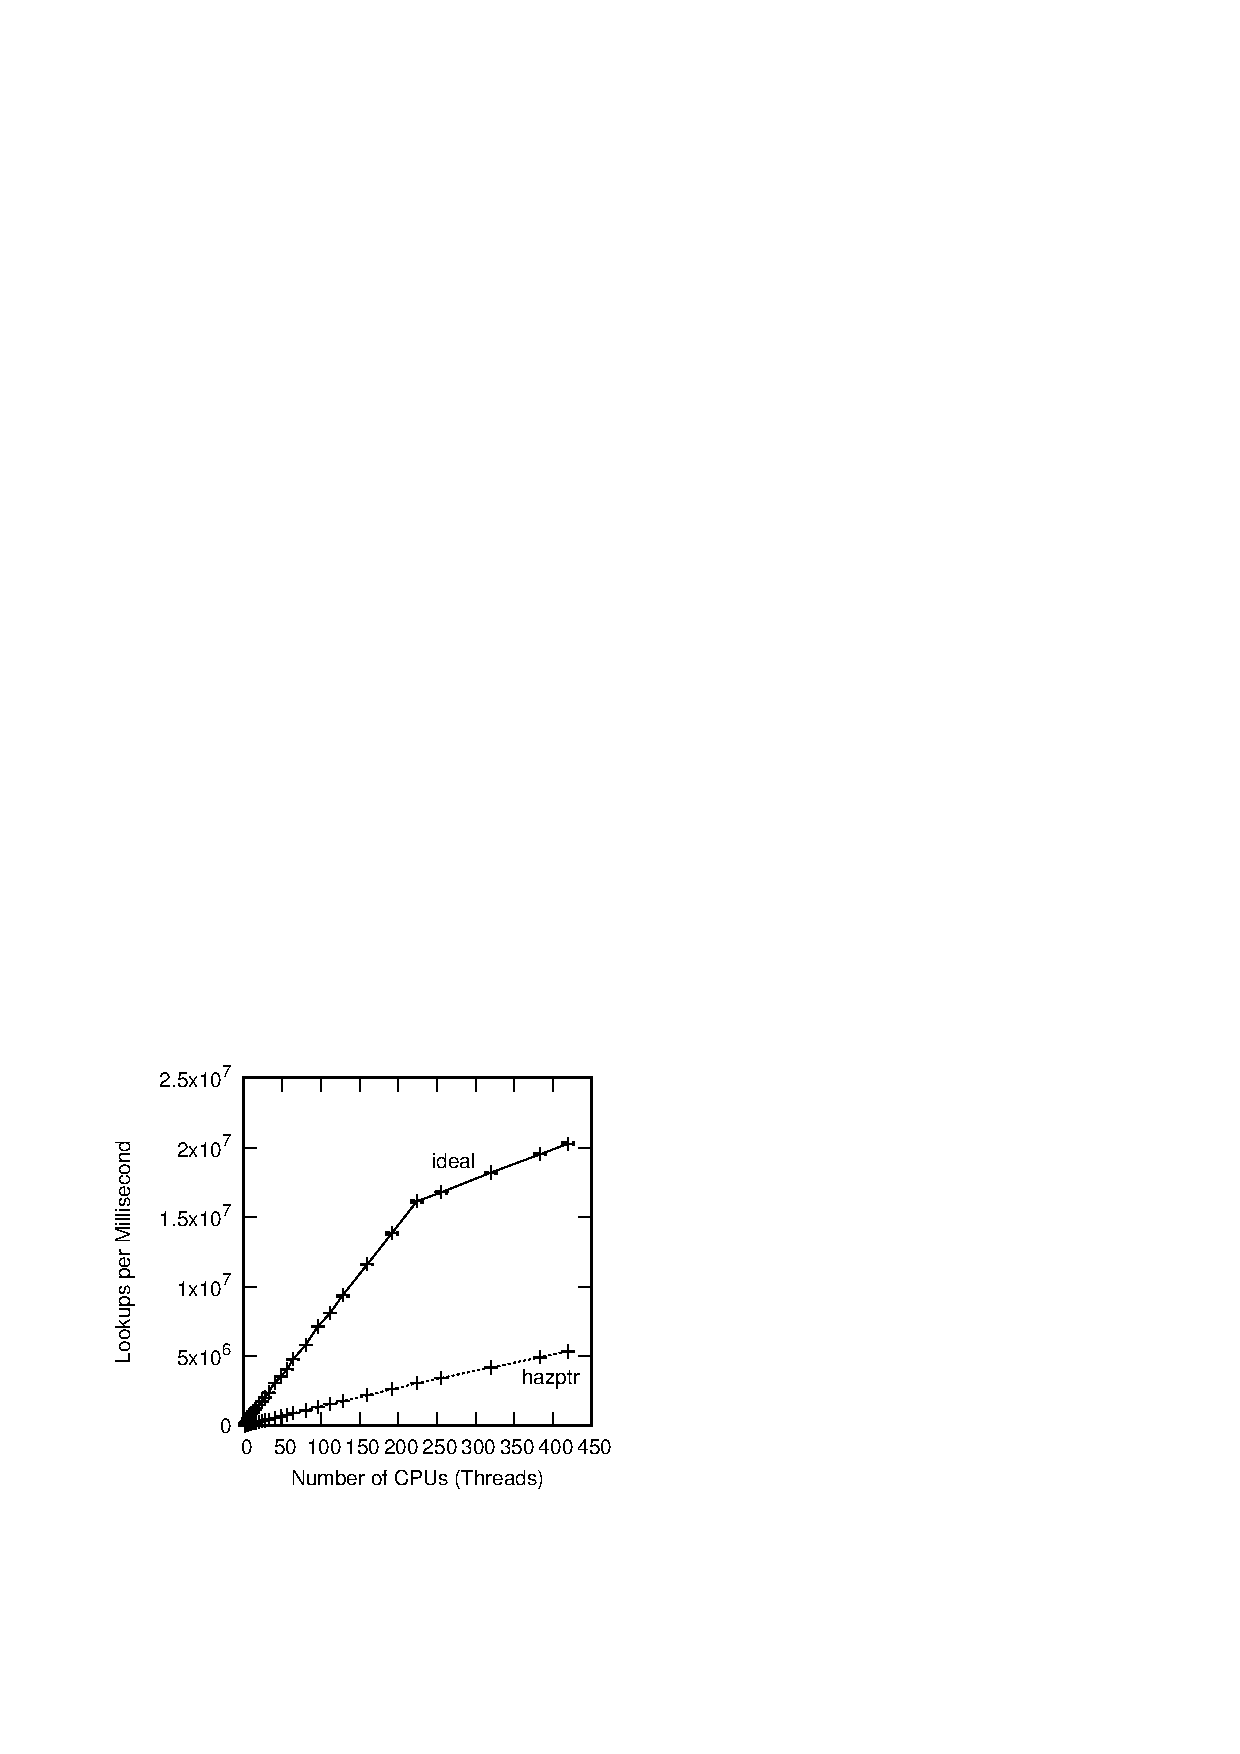
\includegraphics{CodeSamples/defer/perf-hazptr}}
\caption{Pre-BSD Routing Table Protected by Hazard Pointers}
\label{fig:defer:Pre-BSD Routing Table Protected by Hazard Pointers}
\end{figure}

Figure~\ref{fig:defer:Pre-BSD Routing Table Protected by Hazard Pointers}
shows the hazard-pointers-protected Pre-BSD routing algorithm's
performance on the same read-only workload as for
Figure~\ref{fig:defer:Pre-BSD Routing Table Protected by Reference Counting}.
Although hazard pointers scale far better than does reference counting,
hazard pointers still require readers to do writes to shared
memory (albeit with much improved locality of reference),
and also require a full memory barrier and retry check for each
object traversed.
Therefore, hazard-pointers performance is still far short of ideal.
On the other hand, unlike naive approaches to concurrent
reference-counting, hazard pointers not only operate correctly for
workloads involving concurrent updates, but also exhibit excellent
scalability.
Additional performance comparisons with other mechanisms may be found in
Chapter~\ref{chp:Data Structures}
and in other publications~\cite{ThomasEHart2007a,McKenney:2013:SDS:2483852.2483867,MagedMichael04a}.

\QuickQuizSeries{%
\QuickQuizB{
	Figure~\ref{fig:defer:Pre-BSD Routing Table Protected by Hazard Pointers}
	shows no sign of hyperthread-induced flattening at 224 threads.
	Why is that?
}\QuickQuizAnswerB{
	Modern microprocessors are complicated beasts, so significant
	skepticism is appropriate for any simple answer.
	That aside, the most likely reason is the full memory barriers
	required by hazard-pointers readers.
	Any delays resulting from those memory barriers would make time
	available to the other hardware thread sharing the core, resulting
	in greater scalability at the expense of per-hardware-thread
	performance.
}\QuickQuizEndB
%
\QuickQuizE{
	The paper ``Structured Deferral: Synchronization via
	Procrastination''~\cite{McKenney:2013:SDS:2483852.2483867}
	shows that hazard pointers have near-ideal performance.
	Whatever happened in
	Figure~\ref{fig:defer:Pre-BSD Routing Table Protected by Hazard Pointers}???
}\QuickQuizAnswerE{
	First,
	Figure~\ref{fig:defer:Pre-BSD Routing Table Protected by Hazard Pointers}
	has a linear y-axis, while most of the graphs in the
	``Structured Deferral'' paper have logscale y-axes.
	Next, that paper uses lightly-loaded hash tables, while
	Figure~\ref{fig:defer:Pre-BSD Routing Table Protected by Hazard Pointers}'s
	uses a 10-element simple linked list, which means that hazard pointers
	face a larger memory-barrier penalty in this workload than in
	that of the ``Structured Deferral'' paper.
	Finally, that paper used an older modest-sized x86 system, while
	a much newer and larger system was used to generate the data
	shown in
	Figure~\ref{fig:defer:Pre-BSD Routing Table Protected by Hazard Pointers}.

	In addition, use of pairwise asymmetric
	barriers~\cite{Windows2008FlushProcessWriteBuffers,JonathanCorbet2010sys-membarrier,Linuxmanpage2018sys-membarrier}
	has been proposed to eliminate the read-side hazard-pointer
	memory barriers on systems supporting this notion~\cite{DavidGoldblatt2018asymmetricFences},
	which might improve the performance of hazard pointers beyond
	what is shown in the figure.

	As always, your mileage may vary.
	Given the difference in performance, it is clear that hazard
	pointers give you the best performance either for
	very large data structures (where the memory-barrier overhead
	will at least partially overlap cache-miss penalties) and
	for data structures such as hash tables where a lookup
	operation needs a minimal number of hazard pointers.
}\QuickQuizEndE
}

The next section attempts to improve on hazard pointers by using
sequence locks, which avoid both read-side writes and per-object memory
barriers.
